\documentclass[tikz,border=2pt]{standalone}
\usepackage{amsmath,amssymb}
\usetikzlibrary{arrows.meta}
\begin{document}
% Two-station open network of Exercise 7.3.3 with alpha = 1/2, beta_1 = beta_2 = 1/4, gamma = 1:
% each arrow out of station i carries the routing probability P_ij, the exit P_20 = 1/2; rows of P
% sum to 1 and 1/2. The traffic equations give lambda_1 = 3, lambda_2 = 2.
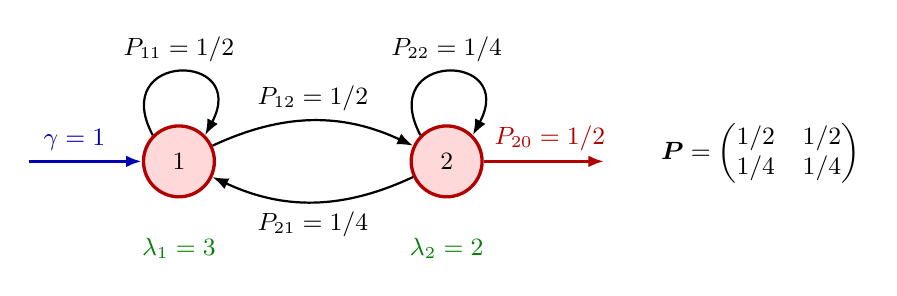
\begin{tikzpicture}[font=\small, >={Latex[length=2mm]}]
  \node[circle, draw=red!70!black, very thick, fill=red!15, minimum size=0.9cm] (s1) at (0,0) {$1$};
  \node[circle, draw=red!70!black, very thick, fill=red!15, minimum size=0.9cm] (s2) at (3.4,0) {$2$};
  % external arrivals
  \draw[->, blue!70!black, very thick] (-1.9,0) -- (s1.west) node[pos=0.4, above] {$\gamma=1$};
  % routing
  \draw[->, thick] (s1) to[bend left=25] node[midway, above] {$P_{12}=1/2$} (s2);
  \draw[->, thick] (s2) to[bend left=25] node[midway, below] {$P_{21}=1/4$} (s1);
  \draw[->, thick] (s1.north west) .. controls (-0.9,1.4) and (0.9,1.4) .. (s1.north east)
    node[pos=0.5, above] {$P_{11}=1/2$};
  \draw[->, thick] (s2.north west) .. controls (2.5,1.4) and (4.3,1.4) .. (s2.north east)
    node[pos=0.5, above] {$P_{22}=1/4$};
  % exit
  \draw[->, red!70!black, very thick] (s2.east) -- (5.4,0) node[pos=0.55, above] {$P_{20}=1/2$};
  % rates
  \node[green!50!black, anchor=north] at (0,-0.85) {$\lambda_1=3$};
  \node[green!50!black, anchor=north] at (3.4,-0.85) {$\lambda_2=2$};
  % matrix
  \node[anchor=west] at (6.0,0.1) {$\boldsymbol{P}=\begin{pmatrix}1/2&1/2\\ 1/4&1/4\end{pmatrix}$};
\end{tikzpicture}
\end{document}
